\subsection{Teil 1 - Klassifizierung von Rechnungen}

In diesem Kapitel werden zwei Experimente aufgezeigt, mit welchen die Klassifizierung von Rechnungen ermöglicht werden soll. Die Klassifizierung dient dazu, eine Rechnung einer bestimmten Art (Klasse) zuzuweisen. Die Klassen \enquote{Optiker} und \enquote{Fitness} sind durch die Anforderungen gegeben. Neben diesen Klassen könnten Rechnungen noch in viele weitere Klassen eingeteilt werden. Um die Erweiterbarkeit des Modells um weitere Klassen zu prüfen, wird eine zusätzliche Klasse eingeführt. In diesem Experiment werden Rechnungen in die Klassen \enquote{Optiker}, \enquote{Fitness}, \enquote{Sportverein} und \enquote{Übrige} eingeteilt. In der späteren Anwendung wäre es denkbar, die Anzahl Klassen zu erhöhen und somit auch andere Arten von Rechnungen zu Automatisieren.

Als Ausgangspunkt für die Klassifizierung steht ein Bild einer Rechnung. Die Klassifizierung von Bildern respektive Fotos ist eine bekannte Problematik der Computer Vision und bildet in diesem Bereich die Grundlage für die Lösung vieler weiterer Problematiken~\autocite{StanfordGithubClassification}. 

% Die Wichtigkeit der Bildklassifizierung zeigt die Organisation ImageNet. ImageNet aht es zum Ziel, Forschern einen einfachen Zugang zu Datensätzen von Bildern zu gewähren. Seit 2010 wurden bereits sieben Wettbewerbe im Bereich der Computer Vision veranstaltet rund um die Klassifizierung von Bildern und die Erkennung von Objekten auf diesen Bildern~\autocite{ImageNet2019}. 

Es liegt nahe, die Klassifizierung der Rechnungen mit Bild-basierten Modellen aus dem Bereich der Computer Vision anzugehen. Im folgenden Kapitel wird dieser Ansatz verfolgt.

Nicht nur im Bereich der Computer Vision ist die Problematik der Klassifizierung ein viel behandeltes Themengebiet. Im Bereich des Natural Language Processing ist die Klassifizierung von Wörtern, Sätzen oder ganzen Texten eine bekannte Problemstellung. Die sogenannte Text Classification ist die Grundlage für viele Applikationen, welche mit Texten arbeiten. So verwenden beispielsweise Mail-Server Text Classification um zu entscheiden, ob ein E-Mail Spam ist oder nicht~\autocite{GoogleTextClassification}

Im Kapitel \ref{chap:text-based-classification} wird die Text-basierte Klassifizierung der Rechnungen weiter verfolgt.

Die beiden Vorgehen zur Klassifizierung werden anhand der knapp 24500 bereits bei der AXA eingereichten Rechnungen evaluiert. Um dies zu ermöglichen, wurden die Rechnungen aus dem System der AXA exportiert und manuell in die oben genannten Klassen eingeteilt. 

Der Datensatz musste auf 17196 Rechnungen reduziert werden. Etwas mehr als 7000 Rechnungen hatten mehr als eine Seite. Aus diesem Grund konnten diese Rechnungen mit den vorhandenen Informationen nicht eindeutig einer Klasse zugewiesen werden. Eine manuelle Klassifizierung würde für den Umfang dieses Experiments einen zu grossen Arbeitsaufwand darstellen.

127 Rechnungen wurden aufgrund mangelnder Qualität aussortiert. Diese Problematik wird durch die vor kurzem eingeführte Qualitätsprüfung (vgl. Abbildung \ref{prozessaxa}) nicht mehr vorkommen und ist deshalb für diese Arbeit nicht relevant.

Nach der Einteilung in die vier Klassen ist festzustellen, dass die 17196 Rechnungen eine sehr unregelmässige Verteilung aufweisen (vgl. Abbildung. \ref{class-distribution}). Die Klasse Sportverein ist gegenüber den anderen Klassen mit nur 760 Rechnungen unterrepräsentiert. Die Klasse Übrige ist hingegen mit 12751 Rechnunge überrepräsentiert. Es ist wichtig, diesem Umstand während dem Training eines Modells Rechnung zu tragen. Ansonsten würde die Voraussage des Modells zu Oft in der überrepräsentierten Klasse \enquote{Übrige} resultieren. Diese Problematik kann auf diverse Arten angegangen werden. In dieser Arbeit wird während dem Training die loss Funktion, welche das Modell trainiert, durch eine Gewichtung aufgrund der Klassenverteilung, diesem Umstand Rechnung tragen~\autocite{Buda2018}.

\begin{figure}[h]
    \captionsetup{width=.9\linewidth}
    \caption{Ungleichverteilung der Klassen innerhalb des Trainingsdatensatzes}
    \label{class-distribution}
    \centering
    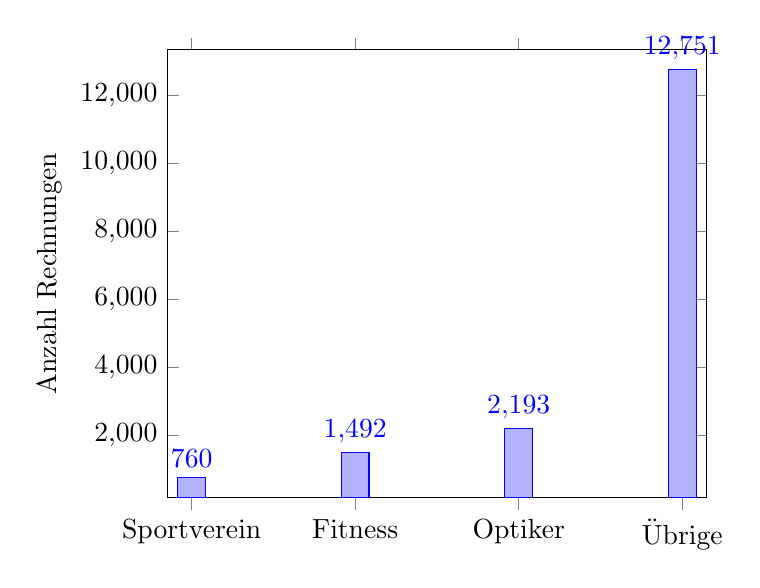
\begin{tikzpicture}
        \begin{axis}[
            ybar,
        	ylabel=Anzahl Rechnungen,
        	enlargelimits=0.05,
            symbolic x coords={Sportverein,Fitness,Optiker,Übrige},
            y tick label style={/pgf/number format/fixed},
            scaled y ticks=false,
            xtick=data,
            nodes near coords,
            nodes near coords align={vertical},
        ]
            \addplot 
        	    coordinates {(Sportverein, 760) (Fitness, 1492) (Optiker, 2193) (Übrige, 12751)};
        \end{axis}
    \end{tikzpicture}
\end{figure}
